\documentclass{TDP003mall}


\newcommand{\version}{Version 1.0}
\author{Adam Ivarsson, \url{adaiv505@student.liu.se}\\
  Lukas Michanek, \url{lukmi182@student.liu.se}}
\title{System Documentation}
\date{2015-10-10}
\rhead{Adam Ivarsson\\
Lukas michanek\\}

\begin{document}
\projectpage

\section{System Documentation}\label{system-documentation}

This document documents the technical structure of our portfolio.

\section{General overview}\label{general-overview}

\centerline{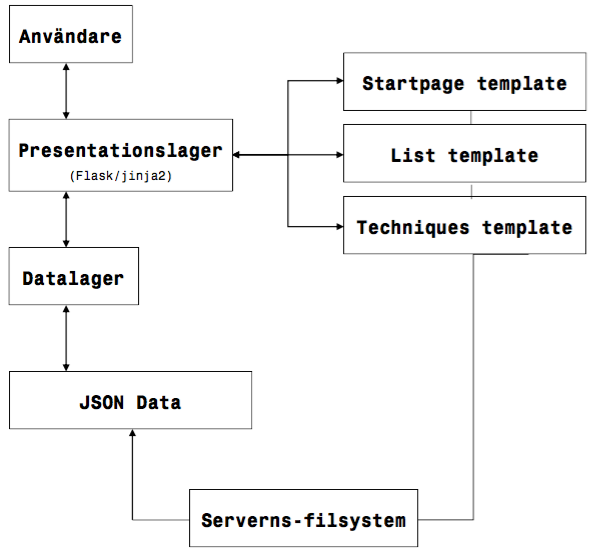
\includegraphics[scale=0.5]{graph_1}}

This application uses quite a simple model. The user makes requests to the web server, which in this case is Flask, and then Flask works with the database to fetch the requested data. Jinja will turn the HTML templates into real HTML documents with the data that Flask got from the data layer, and a response will be made that lets the user see the webpage.

To further understand how this works, please look at the following UML diagram. It specifies in a simplified form what happens when you load and use the `/list` page, the most complicated part of the application.

\centerline{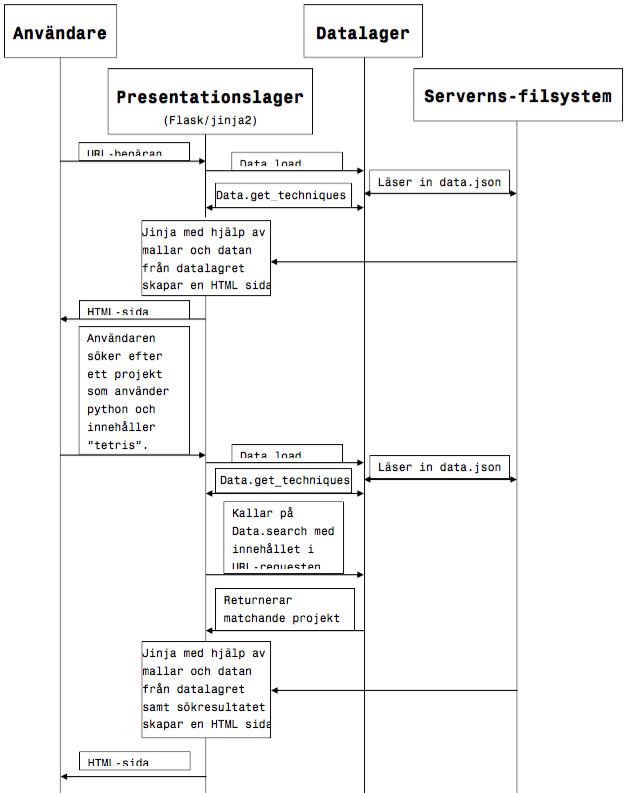
\includegraphics[scale=0.8]{graph_2}}

\section{Presentation-layer functions}\label{presentation-functions}

This is how functions in the presentation layer work:

Flask handels most of the heavy lifting for us, including handling what request get sent to what function. Our functions (and when they are called by Flask) are as follows:

\subsection{request\_logging()} 
Gets called BEFORE each request to the server is handheld. Its function is to logg each request to the server.

\subsection{main\_page()} 
Gets called when the URL `/` is requested. Using the datalayer, Jinja2, and the `main.html` template this function returns the main page of the portfolio to whoever sent the request.

\subsection{list\_page()} 
Gets called when the URL `/list` is requested. Using the datalayer, Jinja2, and the `list.html` template this function EITHER returns the default list page (containing all the projects) OR if it has been requested using a `POST` it instead returns the list page containing a list of projects that fit the search parameters contained in the `POST` request.

\subsection{project\_page(id)}
Gets called when the URL `/project/<id>` is requested, where id is the id of a project. Using the data layer, Jinja2, and the project.html template this function returns a page containing information regarding the project that in the database has the specified id. If the specified project does not exist, it returns the `404` page.

\subsection{technique\_page()} 
Gets called when the  URL `/techniques` is requested. Using the datalayer, Jinja2, and the `techniques.html` template this function returns the techniques page of the portfolio populated with all the techniques found in our datalayer to whoever sent the request.

All web requests and stack traces are also logged to a file on disk for easy debugging. This file contains the same type of information that you'd normally see in the console when running the server.

\section{Error handling}\label{error-handling}
We also have a bit of error handling...

Again, Flask does all the heavy lifting here, and using the same method as for the normal pages we can specify what error calls what function:

\subsection{page\_not\_found(e)} 
This function gets called when flask detects `404` error. Using the datalayer, Jinja2, and the `404.html` template this function returns a basic page informing the user that a `404` error occured. This function is called when the server can't find a page fitting the requested URL (`404`).

\subsection{internal\_error(e)}
This function gets called when flask detects `500` error. Using the datalayer, Jinja2, and the `500.html` template this function returns a basic page informing the user that a `500` error occured.
It also adds alot of usefull information to the logg to help with debuging.
This function is called when there is an internal server error(`500`)

\section{System specifications}\label{system-specs}
The system was built to comply with this system specification: \url{https://www.ida.liu.se/~TDP003/current/resources/TDP003_systemspecifikation.pdf}, and additionally, all functions in both the data and presentation layer are documented very well. If you have any doubts what so ever, reading the documented code will probably be of great help to you.

\end{document}

